% Options for packages loaded elsewhere
\PassOptionsToPackage{unicode}{hyperref}
\PassOptionsToPackage{hyphens}{url}
%


\PassOptionsToPackage{table}{xcolor}

\documentclass[
  10pt,
  letterpaper,
]{article}

\usepackage{amsmath,amssymb}
\usepackage{iftex}
\ifPDFTeX
  \usepackage[T1]{fontenc}
  \usepackage[utf8]{inputenc}
  \usepackage{textcomp} % provide euro and other symbols
\else % if luatex or xetex
  \usepackage{unicode-math}
  \defaultfontfeatures{Scale=MatchLowercase}
  \defaultfontfeatures[\rmfamily]{Ligatures=TeX,Scale=1}
\fi
\usepackage{lmodern}
\ifPDFTeX\else  
    % xetex/luatex font selection
    \setmainfont[]{Charter}
\fi
% Use upquote if available, for straight quotes in verbatim environments
\IfFileExists{upquote.sty}{\usepackage{upquote}}{}
\IfFileExists{microtype.sty}{% use microtype if available
  \usepackage[]{microtype}
  \UseMicrotypeSet[protrusion]{basicmath} % disable protrusion for tt fonts
}{}
\makeatletter
\@ifundefined{KOMAClassName}{% if non-KOMA class
  \IfFileExists{parskip.sty}{%
    \usepackage{parskip}
  }{% else
    \setlength{\parindent}{0pt}
    \setlength{\parskip}{6pt plus 2pt minus 1pt}}
}{% if KOMA class
  \KOMAoptions{parskip=half}}
\makeatother
\usepackage{xcolor}
\usepackage[top=0.85in,left=2.75in,footskip=0.75in]{geometry}
\setlength{\emergencystretch}{3em} % prevent overfull lines
\setcounter{secnumdepth}{-\maxdimen} % remove section numbering


\providecommand{\tightlist}{%
  \setlength{\itemsep}{0pt}\setlength{\parskip}{0pt}}\usepackage{longtable,booktabs,array}
\usepackage{calc} % for calculating minipage widths
% Correct order of tables after \paragraph or \subparagraph
\usepackage{etoolbox}
\makeatletter
\patchcmd\longtable{\par}{\if@noskipsec\mbox{}\fi\par}{}{}
\makeatother
% Allow footnotes in longtable head/foot
\IfFileExists{footnotehyper.sty}{\usepackage{footnotehyper}}{\usepackage{footnote}}
\makesavenoteenv{longtable}
\usepackage{graphicx}
\makeatletter
\def\maxwidth{\ifdim\Gin@nat@width>\linewidth\linewidth\else\Gin@nat@width\fi}
\def\maxheight{\ifdim\Gin@nat@height>\textheight\textheight\else\Gin@nat@height\fi}
\makeatother
% Scale images if necessary, so that they will not overflow the page
% margins by default, and it is still possible to overwrite the defaults
% using explicit options in \includegraphics[width, height, ...]{}
\setkeys{Gin}{width=\maxwidth,height=\maxheight,keepaspectratio}
% Set default figure placement to htbp
\makeatletter
\def\fps@figure{htbp}
\makeatother

% Use adjustwidth environment to exceed column width (see example table in text)
\usepackage{changepage}

% marvosym package for additional characters
\usepackage{marvosym}

% cite package, to clean up citations in the main text. Do not remove.
% Using natbib instead
% \usepackage{cite}

% Use nameref to cite supporting information files (see Supporting Information section for more info)
\usepackage{nameref,hyperref}

% line numbers
\usepackage[right]{lineno}

% ligatures disabled
\usepackage{microtype}
\DisableLigatures[f]{encoding = *, family = * }

% create "+" rule type for thick vertical lines
\newcolumntype{+}{!{\vrule width 2pt}}

% create \thickcline for thick horizontal lines of variable length
\newlength\savedwidth
\newcommand\thickcline[1]{%
  \noalign{\global\savedwidth\arrayrulewidth\global\arrayrulewidth 2pt}%
  \cline{#1}%
  \noalign{\vskip\arrayrulewidth}%
  \noalign{\global\arrayrulewidth\savedwidth}%
}

% \thickhline command for thick horizontal lines that span the table
\newcommand\thickhline{\noalign{\global\savedwidth\arrayrulewidth\global\arrayrulewidth 2pt}%
\hline
\noalign{\global\arrayrulewidth\savedwidth}}

% Text layout
\raggedright
\setlength{\parindent}{0.5cm}
\textwidth 5.25in 
\textheight 8.75in

% Bold the 'Figure #' in the caption and separate it from the title/caption with a period
% Captions will be left justified
\usepackage[aboveskip=1pt,labelfont=bf,labelsep=period,justification=raggedright,singlelinecheck=off]{caption}
\renewcommand{\figurename}{Fig}

% Remove brackets from numbering in List of References
\makeatletter
\renewcommand{\@biblabel}[1]{\quad#1.}
\makeatother

% Header and Footer with logo
\usepackage{lastpage,fancyhdr}
\usepackage{epstopdf}
%\pagestyle{myheadings}
\pagestyle{fancy}
\fancyhf{}
%\setlength{\headheight}{27.023pt}
%\lhead{\includegraphics[width=2.0in]{PLOS-submission.eps}}
\rfoot{\thepage/\pageref{LastPage}}
\renewcommand{\headrulewidth}{0pt}
\renewcommand{\footrule}{\hrule height 2pt \vspace{2mm}}
\fancyheadoffset[L]{2.25in}
\fancyfootoffset[L]{2.25in}
\lfoot{\today}
\makeatletter
\@ifpackageloaded{tcolorbox}{}{\usepackage[skins,breakable]{tcolorbox}}
\@ifpackageloaded{fontawesome5}{}{\usepackage{fontawesome5}}
\definecolor{quarto-callout-color}{HTML}{909090}
\definecolor{quarto-callout-note-color}{HTML}{0758E5}
\definecolor{quarto-callout-important-color}{HTML}{CC1914}
\definecolor{quarto-callout-warning-color}{HTML}{EB9113}
\definecolor{quarto-callout-tip-color}{HTML}{00A047}
\definecolor{quarto-callout-caution-color}{HTML}{FC5300}
\definecolor{quarto-callout-color-frame}{HTML}{acacac}
\definecolor{quarto-callout-note-color-frame}{HTML}{4582ec}
\definecolor{quarto-callout-important-color-frame}{HTML}{d9534f}
\definecolor{quarto-callout-warning-color-frame}{HTML}{f0ad4e}
\definecolor{quarto-callout-tip-color-frame}{HTML}{02b875}
\definecolor{quarto-callout-caution-color-frame}{HTML}{fd7e14}
\makeatother
\makeatletter
\@ifpackageloaded{caption}{}{\usepackage{caption}}
\AtBeginDocument{%
\ifdefined\contentsname
  \renewcommand*\contentsname{Table of contents}
\else
  \newcommand\contentsname{Table of contents}
\fi
\ifdefined\listfigurename
  \renewcommand*\listfigurename{List of Figures}
\else
  \newcommand\listfigurename{List of Figures}
\fi
\ifdefined\listtablename
  \renewcommand*\listtablename{List of Tables}
\else
  \newcommand\listtablename{List of Tables}
\fi
\ifdefined\figurename
  \renewcommand*\figurename{Figure}
\else
  \newcommand\figurename{Figure}
\fi
\ifdefined\tablename
  \renewcommand*\tablename{Table}
\else
  \newcommand\tablename{Table}
\fi
}
\@ifpackageloaded{float}{}{\usepackage{float}}
\floatstyle{ruled}
\@ifundefined{c@chapter}{\newfloat{codelisting}{h}{lop}}{\newfloat{codelisting}{h}{lop}[chapter]}
\floatname{codelisting}{Listing}
\newcommand*\listoflistings{\listof{codelisting}{List of Listings}}
\makeatother
\makeatletter
\makeatother
\makeatletter
\@ifpackageloaded{caption}{}{\usepackage{caption}}
\@ifpackageloaded{subcaption}{}{\usepackage{subcaption}}
\makeatother

\ifLuaTeX
  \usepackage{selnolig}  % disable illegal ligatures
\fi
\usepackage[numbers,square,comma]{natbib}
\bibliographystyle{plos2015}
\usepackage{bookmark}

\IfFileExists{xurl.sty}{\usepackage{xurl}}{} % add URL line breaks if available
\urlstyle{same} % disable monospaced font for URLs
\hypersetup{
  pdftitle={Recommendations for reporting epidemiological parameters},
  pdfauthor={Joshua W. Lambert; Carmen Tamayo; Sangeeta Bhatia; Ruth McCabe; Gina Cuomo-Dannenburg; Adam Kucharski; Anne Cori},
  pdfkeywords={epidemiological parameters, reporting guidelines},
  hidelinks,
  pdfcreator={LaTeX via pandoc}}




\begin{document}
\vspace*{0.2in}

% Title must be 250 characters or less.
\begin{flushleft}
{\Large
\textbf\newline{Recommendations for reporting epidemiological
parameters} % Please use "sentence case" for title and headings (capitalize only the first word in a title (or heading), the first word in a subtitle (or subheading), and any proper nouns).
}
\newline
\\
% Insert author names, affiliations and corresponding author email (do not include titles, positions, or degrees).
Joshua W. Lambert\textsuperscript{1*}, Carmen
Tamayo\textsuperscript{1}, Sangeeta Bhatia\textsuperscript{2,3}, Ruth
McCabe\textsuperscript{2}, Gina
Cuomo-Dannenburg\textsuperscript{2}, Adam
Kucharski\textsuperscript{1}, Anne Cori\textsuperscript{2}
\\
\bigskip
\textbf{1} London School of Hygiene and Tropical
Medicine, \\ \textbf{2} Imperial College London, \\ \textbf{3} UK Health
Security Agency, 
\bigskip

% Insert additional author notes using the symbols described below. Insert symbol callouts after author names as necessary.
% 
% Remove or comment out the author notes below if they aren't used.
%
% Primary Equal Contribution Note
\Yinyang These authors contributed equally to this work.

% Additional Equal Contribution Note
% Also use this double-dagger symbol for special authorship notes, such as senior authorship.
%\ddag These authors also contributed equally to this work.

% Current address notes
\textcurrency Current Address: Dept/Program/Center, Institution Name, City, State, Country % change symbol to "\textcurrency a" if more than one current address note
% \textcurrency b Insert second current address 
% \textcurrency c Insert third current address

% Deceased author note
\dag Deceased

% Group/Consortium Author Note
\textpilcrow Membership list can be found in the Acknowledgments section.

% Use the asterisk to denote corresponding authorship and provide email address in note below.
* joshua.lambert@lshtm.ac.uk

\end{flushleft}



\linenumbers

Epidemiological parameters are a necessity in understanding the spread
of infectious disease; from the rate of transmission, to severity, to
serology, these parameters underline our ability to quantify and respond
to disease outbreaks. The estimation of epidemiological parameters has a
long history in epidemiology and the models and methods applied have
become more complex; and with this complexity comes the numerous ways
parameters can be reported in the literature. Here we provide guidance
on how to clearly communicate estimated epidemiological parameters, to
maximise their secondary use and minimise possible human errors that
come with extracting parameters from the literature and applying them in
their own epidemiological analysis. Our aim is for future work that
reports epidemiological parameters to be consistent, reproducible and
comparable.

\subsection{Introduction}\label{introduction}

Epidemiological parameters are quantities that characterise the spread
of infectious diseases, their epidemiological outcomes and temporal
information on dynamics of disease progression and transmission
\citep{coriInferenceEpidemicDynamics2024}. They are critical to
understand epidemic and pandemic dynamics and respond accordingly
\citep{polonskyOutbreakAnalyticsDeveloping2019}. Most epidemiological
parameters take the form of distributions because there is inherent
variability in the epidemiological characteristics being measured. An
illustration is the delay from infection to symptom onset. The
variability of individuals in immune response and variability of the
infectious agent in pathology are two ways, among many others, that lead
to some individuals having shorter time delay between infection and
onset of symptoms. Due to most epidemiological parameters being
described by distributional forms they are estimated by fitting
distributions to epidemiological data on cases or contacts.

It has become general practice that when epidemiological parameters are
required, either for analyses of epidemiological case data or to make
policy decisions like quarantine duration, that the literature is
searched to find a suitable peer-reviewed publication reporting the
parameter needed. However, this process has several limitations. The
time requirement to search through papers to find the highest quality
epidemiological parameter means that in time-limited scenarios, for
example early in an outbreak when the situation is evolving rapidly and
new data is continually gathered, a suboptimal parameter set may be
extracted and used. This has lead to previous \emph{ad hoc} reviews of
epidemiological parameters for specific pathogens (e.g.~Ebola
\citep{vankerkhoveReviewEpidemiologicalParameters2015a}). The choice of
parameter is also likely to be somewhat subjective without a clear
quality assurance framework to evaluate and compare different parameter
estimates. The manual extraction of copying and pasting parameters out
of the literature comes with the risk of discrepancies entering the
calculations.

Epidemiological parameters have been reported for many diseases and the
data used to infer parameter estimates and the methods of inference
vary.

Efforts to compile a centralised database of epidemiological parameters
have highlighted the variability and ambiguity in parameter reporting
which can lead to uncertainty around what is being reported and how
these epidemiological parameters can be applied in other epidemiological
analyses {[}\citet{cuomo-dannenburgMarburgVirusDisease2024};
doohanLassaFeverOutbreaks2024; \citet{nashEbolaVirusDisease2024}{]}.

This paper was motivated by several research groups independently
attempting to compile a comprehensive library of epidemiological
parameters which could serve as a public resource to easily search,
filter and extract parameters. These groups gathered for a workshop
convened by the World Health Organisation (WHO) Collaboratory in Spring
2024, in which a Global Repository of Epidemiological Parameters (GREP)
was discussed, as well as ideas for guidance on reporting
epidemiological parameters. The guidelines and examples of incorrect
reporting and use were subsequently further developed and resulted in
this paper.

This guidance on reporting of epidemiological parameters does not cover
or advise on estimation methods. Our focus is on the reporting of
parameters post-inference and the benefits of reporting standardisation
on the reuse of epidemiological parameters by those involved in epidemic
or humanitarian response. For guidance on methodologies to use when
inferring delay distributions see
\citet{parkEstimatingEpidemiologicalDelay2024} and
\citet{charnigaBestPracticesEstimating2024}.

Here we focus on the bias caused by badly reported epidemiological
parameters on simple epidemic methods, sometimes referred to as outbreak
analytics \citep[sensu][]{polonskyOutbreakAnalyticsDeveloping2019}, to
showcase the erroneous conclusions that can arise when using parameter
estimates from the literature. The biases produce here will likely
extrapolate to more complex epidemiologilogical modelling. Reporting
guidelines can ensure standardised reporting becomes more commonplace,
which can make it easier to review, summarise and aggregate
epidemiological parameters. We hope that this paper, alongside other
works on reporting best practises in epidemiology
\citep{pollettRecommendedReportingItems2021, charnigaBestPracticesEstimating2024}
enhance the interoperability of research outputs and inputs.

\subsection{Guidance}\label{guidance}

\subsubsection{Parameter inference
reporting}\label{parameter-inference-reporting}

\paragraph{Parameterisation of
distributions}\label{parameterisation-of-distributions}

Many distributions have standard parameterisations. In other words, they
have one, two or in some cases three parameters that are denoted by a
name and often have a greek letter for shorthand. An example of this is
the Gamma distribution which has the parameterisation shape (\(\alpha\))
and rate (\(\beta\)). However, there are often alternative
parameterisations, for the Gamma distribution this is shape (\(k\)) and
scale (\(\theta\)). If left unspecified, the reported parameters may
correspond to different parameters depending on interpretation. Another
example of ambiguous reporting of distribution estimates is when the
parameters and summary statistics have similar names. This is the case
for the lognormal distribution, whose common parameterisation is meanlog
(\(\mu\)) and sdlog (\(\sigma\)) and common summary statistics reported
for a distribution are mean and standard deviation (sd), this is further
confused as both use the same greek letters. Therefore, it is possible
to mistake the reporting of one set of these for the other. Both types
of misinterpretation outlined here can result in substantial differences
in the distributions (Figure 1).

\emph{Guidance}:

\begin{itemize}
\tightlist
\item
  Provide the formula for the Probability Density Function (PDF), or
  Probability Mass Function (PMF) if discrete, in the text or
  supplementary material.
\item
  Clearly report which distribution parameterisation was used to
  estimate parameters and provide parameter names in the text.
\item
  Share code used to estimate parameter(s) for others to reproduce and
  audit methods.
\end{itemize}

\begin{figure}[H]

\centering{

\centering{

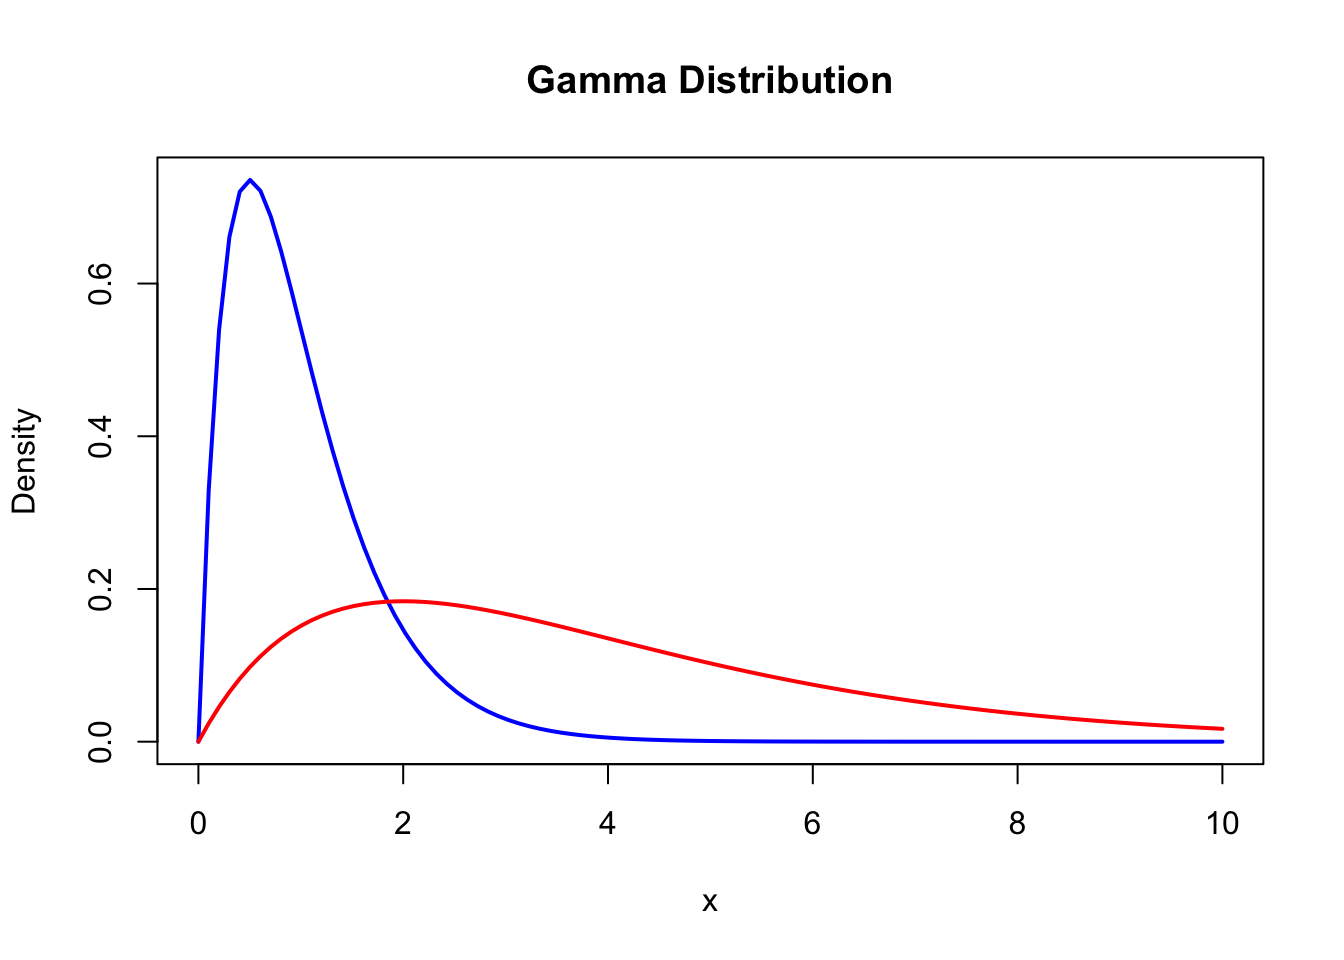
\includegraphics{index_files/figure-latex/use_cases-dist_params-fig-dist-params-output-1.png}

}

\subcaption{\label{fig-dist-params-1}Differences in distributions when
misinterpreting the estimated parameters. (a) Two gamma distributions,
the blue shows a gamma distribution with shape (\(\alpha\)) and rate
(\(\beta\)) of 2, the red shows a gamma distribution with shape (\(k\))
and scale (\(\theta\)) of 2. The rate is the reciprocal of the scale
(\(\beta\) = 1/\(\theta\)), but it is clear from the left hand plot that
misinterpreting the parameter leads to a vastly different distribution
density. (b) Two lognormal distributions, the orange shows the density
of a lognormal distribution with meanlog (\(\mu\)) and sdlog
(\(\sigma\)) of 0.5, and the green with the meanlog and sdlog of 1.87
and 1.00, respectively (these values are the conversion from meanlog and
sdlog into mean and standard deviation). Again showing how
misinterpreting the parameters can lead to differences in
epidemiological parameters.}

\centering{

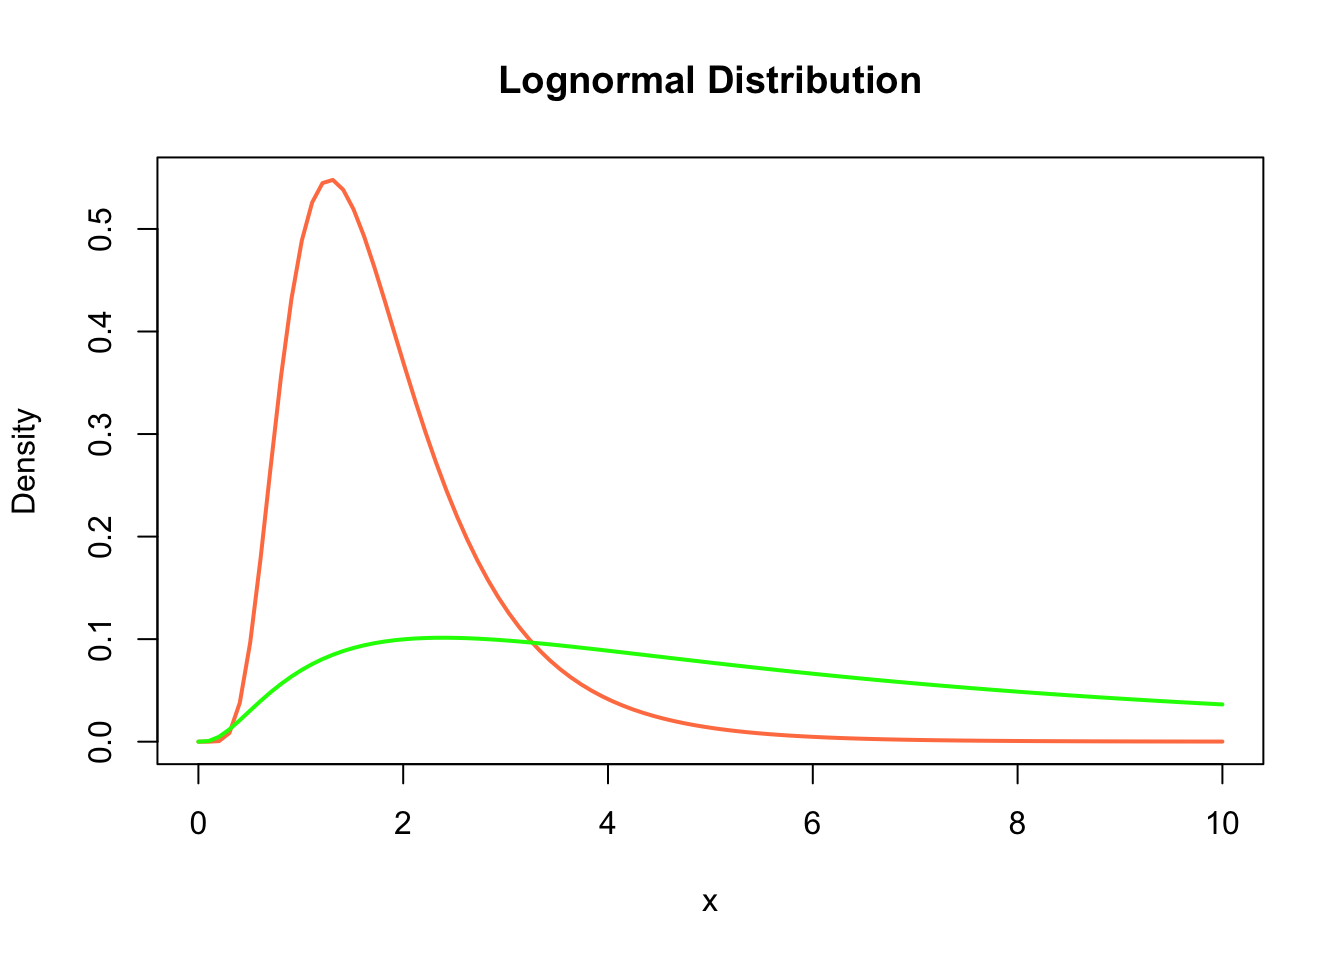
\includegraphics{index_files/figure-latex/use_cases-dist_params-fig-dist-params-output-2.png}

}

\subcaption{\label{fig-dist-params-2}}

}

\caption{\label{fig-dist-params}}

\end{figure}%

\textsubscript{Source:
\href{https://joshwlambert.github.io/epiparameterReportingGuidance/use_cases/dist_params.embed-preview.html\#cell-fig-dist-params}{Define
the x values for the plot}}

\paragraph{Parameter estimates vs summary
statistics}\label{parameter-estimates-vs-summary-statistics}

Instead of reporting the parameter estimates for a parametric
distribution, summary statistics may be provided. In some instances a
set of summary statistics can be analytically converted into
distribution parameters (the specific summary statistics that can be
converted into parameters varies by distribution). In those cases where
analytical conversion can be done there is no loss in parameter estimate
precision, i.e.~summary statistics are sufficient statistics. Commonly
reported sufficient statistics are the mean and standard deviation or
variance of a distribution. However, it can also be the case that
summary statistics that cannot be analytically converted to distribution
parameters are reported, for example the mean or median and the 95th
percentiles of the distribution. In these cases, distribution parameters
require a second estimation using a numerical conversion. Numerical
conversion can introduce more uncertainty and potentially return
erroneous estimates. Below we show an example of the bias and variance
of distribution parameters when numerically converted from summary
statistics\ldots{} (see \{epiparameter\} R package article for full
exploration of bias in numerical conversion).

Epidemiological parameters can be dimensionless quantities, for example
R0 or secondary attack rate, while others have units. It is especially
critical for the accurate reuse of with dimensions parameters that the
units are reported. For parameters with a temporal dimension, such as
delay distributions, the unit of time ensures that distributions fitted
to data on days or weeks can be clearly understood. Another example is
viral load data that can be reported as Ct or log10 RNA copies/ml. Many
epidemiological parameters will have conventional units, for example
incubation period and serial interval in days, or population density in
individuals/km, but if readers have to assume units then
misinterpretation can have consequences for others that apply the
findings in their own work.

\emph{Guidance}:

\begin{itemize}
\tightlist
\item
  Report the estimated distribution parameters first and foremost before
  optionally reporting summary statistics. This will avoid any secondary
  estimation step which can introduce unwanted and unnecessary bias.
\item
  If a parameter has a unit, report this with the estimates, ensuring it
  matches the data of input of the model.
\end{itemize}

\begin{tcolorbox}[enhanced jigsaw, breakable, rightrule=.15mm, leftrule=.75mm, left=2mm, colframe=quarto-callout-tip-color-frame, toprule=.15mm, bottomrule=.15mm, opacityback=0, colback=white, arc=.35mm]

\vspace{-3mm}\textbf{Use case: Severity}\vspace{3mm}

\textbf{Use case: Ambiguous reporting of onset-to-death delay
distribution and erroneous CFR estimates}

In a scenario in which the case fatality risk (CFR) needs to be
calculated for an ongoing, growing disease outbreak an onset-to-death
delay distribution is required to calculate an unbiased CFR estimate,
due to some individuals being infected but theiry outcome (i.e recovery
or death) is unknown \citet{nishiuraEarlyEpidemiologicalAssessment2009}.

A line list of the current outbreak is available, but no estiates of the
onset-to-death delay are available for this outbreak and there is not
enough case data to reliably estimate it from the line list. Therefore a
previously inferred onset-to-death distribution is searched and
extracted from the literature for the same pathogen from a past
outbreak.

The paper reporting the onset-to-death states:

\begin{quote}
``\ldots{} the average duration between the time when symptoms first
appeared and death of the patients was estimated. The mean
onset-to-death delay was of 14.5 days, with a standard deviation of
6.7.''
\end{quote}

The ambiguous reporting of the esimates means the onset-to-death delay
can be (mis)interpreted in several ways. The paper is reporting the
summary statistics mean and standard deviation for a lognormal
distribution they fitted to the data. The estimates could be
misinterpreted as meanlog and sdlog do the lognormal distribution, or
could be misinterpreted as the summary statistics of the raw data
(i.e.~sample statistics). The CFR calculation for an unbiased estimate
requires a parametric probability density/mass function. Therefore,
given the ambiguity we demonstrate the correct interpretation and three
misinterpretations of the reported onset-to-death and show how the CFR
varies as a result. We use the \{simulist\} and \{cfr\} R packages to
simulate line list data and calculate the CFR, respectively
\citet{lambertSimulistSimulateDisease2024} and
\citet{gupteCfrEstimateDisease2024}.

\textsubscript{Source:
\href{https://joshwlambert.github.io/epiparameterReportingGuidance/index.qmd.html}{Article
Notebook}}

\textsubscript{Source:
\href{https://joshwlambert.github.io/epiparameterReportingGuidance/index.qmd.html}{Article
Notebook}}

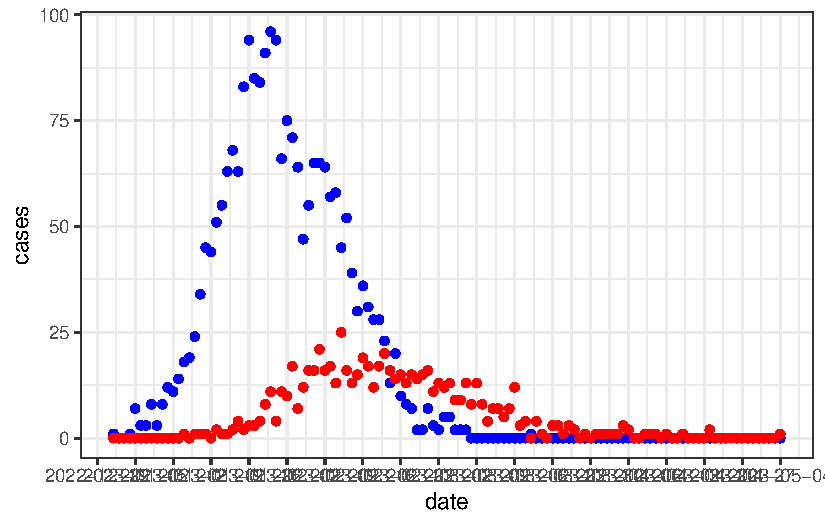
\includegraphics{index_files/figure-pdf/unnamed-chunk-3-1.pdf}

\textsubscript{Source:
\href{https://joshwlambert.github.io/epiparameterReportingGuidance/index.qmd.html}{Article
Notebook}}

\textsubscript{Source:
\href{https://joshwlambert.github.io/epiparameterReportingGuidance/index.qmd.html}{Article
Notebook}}

\textsubscript{Source:
\href{https://joshwlambert.github.io/epiparameterReportingGuidance/index.qmd.html}{Article
Notebook}}

\textsubscript{Source:
\href{https://joshwlambert.github.io/epiparameterReportingGuidance/index.qmd.html}{Article
Notebook}}

The correct interpretation can analytically convert the mean and
standard deviation to the lognormal distribution parameters (\(\mu\) =
2.86, \(\sigma\) = 0.53) and parameterise the onset-to-death, resulting
in a CFR of 0.3042, or 30.42\%. Misinterpreting the estimates to be the
lognormal parameters results in an overestimated CFR of NA. Assuming
that the reported estimates are sample summary statistics, the
distribution can be assumed, here we test the assumption that it is a
lognormal (correct assumption) and a gamma distribution (incorrect
assumption). The assumed parametric distribution form can be used to
simulate a sample and the same distribution can be fit to that sample to
estimate the parameters. In the case of assuming a lognormal
distribution the CFR is estimated as 0.2681, whereas assuming a gamma
distribution results in a CFR of 0.2426. The estimated CFR is biased in
both cases but more so when the distribution is assumed incorrectly.

\end{tcolorbox}

\paragraph{Parameter uncertainty vs sample
variability}\label{parameter-uncertainty-vs-sample-variability}

The reporting of distributions is to encapsulate the variability of
epidemiological delays, transmission, severity and others. However,
there is also uncertainty around the parameters estimated. If it is not
clearly stated that a distribution was fit to the data, it can be
unclear whether the uncertainty around the mean corresponds to variation
in the epidemiological case data, i.e.~differences between individuals
resulting in a distribution, or to the confidence or credible interval
around the estimated mean.

\paragraph{Reporting inference method}\label{reporting-inference-method}

The inference method used to infer epidemiological parameters and the
uncertainty that is coupled with those estimates is also important to
report precisely for it to be used in downstream analyses. One common
distinction that can be made between inference method is whether it uses
Maximum likelihood estimation (MLE) or Bayesian estimation. The
resulting uncertainty of parameters, confidence intervals (CI) for MLE
and credible intervals (CrI) for Bayesian fitting, cannot be interpreted
or applied interchangeably \citep{moreyFallacyPlacingConfidence2016}.
Therefore if wanting to propagate uncertainty in parameter estimates,
incorrectly treating CI as CrI or vice versa will lead to bias.

Reporting on Bayesian fitting also has several summary statistics to
describe the central tendency of the inferred posterior sample, for
example, mean, median, mode. It is beneficial for the specific central
tendency statistic used to be explicitly stated.

\emph{Guidance}:

\begin{itemize}
\tightlist
\item
  Report distribution parameters with uncertainty if available. This can
  be reporting the confidence interval (CI) or credible interval (CrI)
  making it clear
\item
  When using Bayesian inference, specifying methods used for posterior
  distribution and making posterior sample openly available via data
  sharing platform, e.g., Zenodo, Data Dryad.
\end{itemize}

The types of distributions commonly fit to estimate delay distributions,
such as serial interval, onset-to-event and incubation period, are
Gamma, lognormal and Weibull. These are used as they are strictly
positive (sometimes offsets or other distributions are used to account
for negative serial intervals (Prete Jr.~et al., 2021)) and are
right-skewed, meaning that most of the distribution mass (i.e.~area
under the curve) is the left of the mean (Figure 1). It is best practice
to fit multiple distributions to the data and compare models using
likelihoods, information criteria or likelihood ratio tests. By
reporting these comparisons with each set of estimated parameters it
allows others to use the distribution they choose while also being aware
of the goodness-of-fit if choosing the non-best-fitting distribution.

\emph{Guidance}:

\begin{itemize}
\tightlist
\item
  If multiple distributions are fit to the raw case data, report the
  goodness-of-fit (e.g.~maximum likelihood, Akaike Information
  Criterion) and the parameter estimates of each distribution either in
  the main text or in the supplementary material.
\end{itemize}

\subsubsection{Contextual information and
metadata}\label{contextual-information-and-metadata}

Since pathogen transmission and spread is known to be affected by
socioeconomic, demographic, and climatic factors, reporting relevant
contextual information alongside parameter estimates is crucial to
understand the circumstances in which these estimates were obtained.
Doing so will allow external readers to make informed decisions about
the generalisability of the reported parameters and usability in their
own analyses.

An important contextual element is detailed information about the sample
population from which parameters were estimated, including factors such
as the geographic location, age distribution, and comorbidities. This is
particularly relevant in those studies where only a specific subset of
the population was sampled, such as health-care workers, pregnant
individuals, or immunocompromised patients.

Other relevant details of the study, such as the type of design and
sampling strategy, should not be overlooked, when reporting
epidemiological parameters, as these provide relevant contextual
information to assess the representativeness of the data and validity of
the statistical methods applied. For instance, methods for estimating
parameters like the serial interval require considering data collection
methods, as different adjustments for biases are needed depending on
whether data on transmission pairs was conducted prospectively or
retrospectively (see section 1.5). The specific case definition used to
estimate parameters should also be reported, where possible, given the
range of clinical signs that many diseases exhibit at different stages
of infection, which can have an impact on the estimation of parameters
like the incubation period or delays from onset to outcome.

Where parameters are reported or inferred during an active outbreak, we
recommend to provide information about the time into the outbreak since
the first case was reported and epidemic phase at the time of the
analysis, especially when inferring delay distributions (see section
1.5). Further contextual information is also relevant for a nuanced
understanding of how parameter estimates may change throughout an
outbreak, e.g., due to changes in containment measures, therapeutics and
vaccination, or volume of testing. For instance, advancements in the
therapeutic approach to critical care patients resulted in a
significantly higher delay from onset to death for COVID-19 patients
during the summer of 2020 (mean of 24.7 days), compared to the first
wave of the pandemic (mean of 19.6 days) (Ward and Johnsen, 2021, PLoS).

Contextual information about the disease's causative agent should also
be reported, including pathogen name, and, where applicable, its type,
subtype and/or strain. This information is relevant, as the
transmissibility, pathogenicity and severity of disease, and their
resulting epidemiological parameters often vary across strains of the
same pathogen. For instance, the incubation period for Influenza type A
is reportedly longer on average than that of Influenza type B, with a
median of 1.4 and 0.6 days, respectively (Lessler, 2009). If the
causative agent is unknown to the authors, either due to it being a
novel pathogen, or simply because this information is not available,
this should be explicitly stated in the publication. Beyond details
about the causative agent, authors should also specify the transmission
routes that have been considered when estimating parameters. This is
particularly crucial for zoonotic and vector-borne diseases, where
explicit clarification is needed on whether the estimates account for
human-to-human transmission only, or if animal-to-human or
vector-to-human transmission is also accounted for.

\emph{Guidance}:

\begin{itemize}
\tightlist
\item
  Provide demographic information about the population and for the
  sample that was used to estimate epidemiological parameters.
\item
  Specify whether analyses were stratified by certain groups, e.g., by
  age, or conducted using data for the whole population.
\item
  Indicate whether reported parameters were obtained during an ongoing
  outbreak and, if so, provide information on the epidemic phase and
  time since outbreak was first declared.
\item
  Clearly state whether variant(s) of the pathogen of interest is known
  and, if so, report the name of the variant and how this was
  determined.
\item
  Specify which transmission pathways of disease were considered, e.g.,
  human-to-human only, or including animal-to-human transmission.
\end{itemize}

\subsubsection{Open science and reproducibility to enhance
reuse}\label{open-science-and-reproducibility-to-enhance-reuse}

The complexities involved in estimating and reporting epidemiological
parameters mean that it is unlikely that all methodological aspects and
considerations can be documented in the paper or even supplementary
material. By sharing data and code it enables reproducibility and
auditing of the methods used. Sharing the code used to infer an
epidemiological parameter enables others to see which method, as well as
any other packages that were used. There are several platforms that
easily enable code sharing, most common are GitHub, GitLab and
BitBucket. To release the software used and provide a unique identifier
(e.g.~DOI) services like Zenodo, Figshare and Dyrad, this provides a
single referenceable snapshot of the code, removing any issue if the
code changes on, for example GitHub. Following these and other good
practices for code sharing will help others navigate and review the code
(Wilson et al., 2017). Openly sharing code enables others to reproduce
the estimates and verify the estimates. They may also be able to assess
the quality of the methods with respect to the available data and
possible bias-adjustments that may be required when working with
real-time outbreak data (citation needed). Sharing the analysis code can
also resolve ambiguities in parameter reporting. If the parameterisation
of the distribution is unclear from the text (see Section 1) then by
checking parameter arguments in the code clarifies their use.

Sharing the data is as important as sharing the code. By data we mean
the input data (i.e.~outbreak case data) and output data (i.e.~parameter
estimates and fitting metadata). If possible the raw data used to fit a
model to estimate an epidemiological parameter should be openly
available. By sharing the raw data it enables reproducibility of the
analysis used to estimate the epidemiological parameters, but also
allows others to apply different models to the data.

Openly sharing epidemiological data can be restricted by personal
identifiable information (PII) and data usage restrictions. There are
some methods available to enable reproducibility even when the raw data
cannot be shared. Anonymisation, if the personal identifiable
information (PII) is not required by the method to infer the
epidemiological parameter then this information can be removed,
de-identified or anonymised prior to uploading the data (citations
needed). Mock or synthetic data can be generated which has the same
characteristics as the empirical data. This enables the analysis to be
reproduced while removing any risk of identification or leaking personal
information.

The epidemiological parameter output should also be shared in full when
possible. Often if the epidemiological parameter are distribution
parameters these will be reported in the text. But the estimates
correlation matrix, variance-covariance matrix, convergence metrics
(e.g.~\ldots) should be shared. For Bayesian analyses sharing the
posterior distribution is most beneficial for reuse as it allows
researchers to calculate whichever summary metric their use case
requires (e.g.~Highest Posterior Density (HPD) Interval).

\subsubsection{Epidemiological parameter use and disjoint analysis
pipelines}\label{epidemiological-parameter-use-and-disjoint-analysis-pipelines}

The aim of this paper has been to provide a set of reporting guidelines
for epidemiological parameter, with the objective to make reusing them
in other epidemiological analyses more reliable, with examples
showcasing when analysis error can result from erroneous or ambiguous
reporting. This argument is premised on the downstream epidemiological
analysis being disjoint from the estimation of the epidemiological
parameters, in other words the method that uses the parameters to
estimate or infer another aspect of an outbreak does not estimate the
parameters. An example of this is when an previously estimated
generation time, or serial interval as a more commonly available
replacement, is used to estimate the real-time reproduction number. If
the data is available to jointly estimate the generation time or serial
interval with the reproduction number, then this is the statistically
optimal approach. However, for a variety of reasons, primarily model
complexity of joint models leading to mathematical and computations
simplification being required, the disjoint or 2-step analysis procedure
is common (ref). Some models to offer joint estimation given sufficient
data (ref). There have not been many studies exploring the statistical
performance of joint versus disjoint estimation (check this sentence and
find ref). There is another aspect to consider, whether a set of
epidemiological parameters exists where the features of the data
(e.g.~sample size, collection procedure) make it more accurate than the
available at hand. In this scenario even if a joint estimation framework
is available and feasible, it might be better to choose estimated
parameters. The contextual information of the data, such as demography,
geography, and comorbidities of the sample, should also be considered in
such a case as the two groups might not be epidemiologically equivalent.
That is all to say that reporting guidelines are relevant due to the
widespread use of disjoint estimation where clear, ambiguous reporting
with coverage of key piece of statistical and contextual information are
required.

\subsection{Conclusion}\label{conclusion}

\subsection{References}\label{references}


\nolinenumbers
  \bibliography{references.bib}


\end{document}
